%\documentclass[12pt]{article}

%\usepackage{hyperref}
%\usepackage{graphicx}
%\usepackage{float}

%\begin{document}
\section{Wikipedia}
In this section, we will describe each step of the procedure from the Wikipedia data dump to displaying the information on the website.
\begin{figure}[H]
    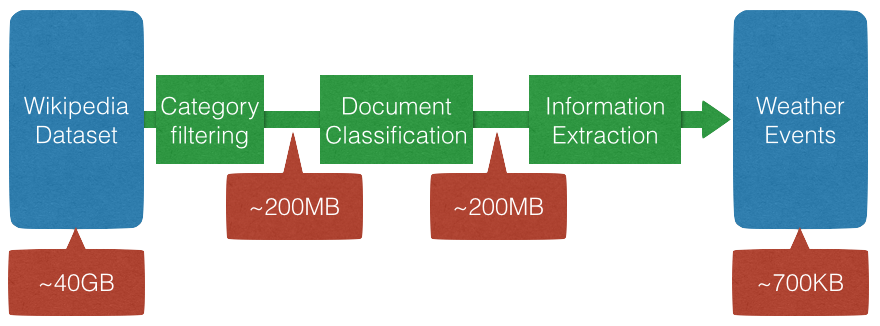
\includegraphics[width=\textwidth]{figures/wiki-flow.png}
    \caption{Overview of Wikipedia information extraction}
     \label{fig:wikiflow}
\end{figure}
\subsection{Available data}
It is possible to download a dump of all English Wikipedia articles, without edit history, from \href{https://meta.wikimedia.org/wiki/Data_dump_torrents#enwiki}{this webpage}. We used the dump from February 3rd, 2014, the latest available when we started the project. It consists of a single XML file which is 10GB compressed, 40GB uncompressed. 
\subsection{Filtering articles}
Obviously, most of Wikipedia articles are irrelevant to our task of find information on weather events, that is why we must first filter the dataset. 
\subsubsection{Filtering based on articles' categories}
The easiest way to prune off topic articles, it to look at their category. Unfortunately, categories on Wikipedia are not hierarchically well organized, so we cannot start from a top category such as ``weather event'' and get a list of every relevant subcategories. Indeed, categories may loop or diverge to another subject.\\\\
Knowing this, we decided to filter categories based on a defined set keywords: "blizzard", "cyclone", "hurricane", "typhoon", "derecho", "drought", "nor'easter", "storm", "tornado", "heat wave", "cold wave", "weather event". \\\\
An article belonging to a category which contains one of keyword is jugged relevant. This allows us to filter out most irrelevant articles, even if there are some false positives (e.g. football players affiliated to a team called ``The Hurricanes'').\\\\
Implementation wise, this filtering consist of a single MapReduce job where the mapper only emit an article if it is relevant, and the reducer combines the articles it receives into a single XML file for each keyword. 
After running the job (usually takes less than 5 minutes), we now only have around 200MB of data, which allows us to do document classification in reasonable time, and filter out the remaining off topic articles.\\ 
We use Mahout's XMLInputFormat which provides an easy way to split the input into multiple articles delimited by the ``$<$article$>$'' and ``$<$/article$>$'' tag and send them to the mapper.
\subsubsection{Filtering using document classification}
ORIANNE
\subsection{Extracting information}
Now that we have only relevant articles, we can start extraction information. \\
The general idea is to first locate the article's infobox which, if it exists, usually provides detailed information on date and location of the event (date formed, date dissipated, areas). If there is no infobox, or we still need more information, we try to extract it from the article's title, and finally, as a last resort we try to find the information in article's body.\\\\
We only use a mapper to extract information, the reducer is only used to combine the results.
After extraction, we have a single CSV file (separated by tabs) containing the following columns: title, category, start date, end date, location. At this point we have $<$1MB of data. Running this job usually takes less than two minutes.
\subsubsection{Extracting dates}
To extract dates we use multiple regexes, to cover the range of available date formats (DD/MM/YYYY; YYYY$|$MM$|$DD; m dd, YYYY; dd m YYYY; etc.). We then convert them all to a predefined date standard: DD/MM/YYYY. 
\subsubsection{Extracting locations}
To extract location, we use a regex based on the lists of continents, countries and american states as well as their corresponding demonyms given in \href{http://en.wikipedia.org/wiki/List_of_adjectival_forms_of_place_names}{this Wikipedia article}.
\subsection{Displaying information}
In order to display correctly the information, we first run a small python that creates http link for each article's title ($<$a href='http://en.wikipedia.org/wiki/\$TITLE'$>$ \$TITLE $<$/a$>$), and get the number of references of an articles from Wikipedia using a GET request (https://en.wikipedia.org/wiki/Special:WhatLinksHere/\$TITLE).\\
We then sort the articles by their number of reference, to display most important events first\\\\
On the webpage, we display the information as an HTML table whose rows can be easily filtered to show only relevant events.
%\end{document}
